% ===================================================================
%  Week 13 — Convolutional Neural Networks
%  Session 1 of 2: From hand-designed kernels to a learned CNN
% ===================================================================
\documentclass[10pt,aspectratio=169]{beamer}
% ===================================================================
%  Shared Beamer preamble for "Practical Image Processing"
%  English slides. Compile with pdfLaTeX.
% ===================================================================

\usetheme{metropolis}
\usepackage[T1]{fontenc}
\usepackage[utf8]{inputenc}
\usepackage{lmodern}
\usepackage{listings}
\usepackage{tcolorbox}
\usepackage{fontawesome5}
\usepackage{booktabs}
\usepackage{amsmath,amssymb}
\usepackage{tikz}
\usepackage{pgfplots}
\pgfplotsset{compat=1.17}
\usetikzlibrary{arrows.meta,positioning,shapes.geometric,fit,backgrounds,matrix}
\tcbuselibrary{skins,breakable}

% ---- Palette --------------------------------------------------------
\definecolor{coursePrimary}{HTML}{1B4965}   % deep blue
\definecolor{courseAccent}{HTML}{E76F51}    % coral
\definecolor{courseGood}{HTML}{2A9D8F}      % teal
\definecolor{courseBad}{HTML}{C0392B}       % red
\definecolor{courseInfo}{HTML}{2980B9}      % blue
\definecolor{codeBg}{HTML}{F5F6FA}
\definecolor{codeKw}{HTML}{8E44AD}
\definecolor{codeStr}{HTML}{2A9D8F}
\definecolor{codeCom}{HTML}{7F8C8D}

\setbeamercolor{frametitle}{bg=coursePrimary}
\setbeamercolor{progress bar}{fg=courseAccent}
\setbeamercolor{alerted text}{fg=courseAccent}
\metroset{block=fill,sectionpage=progressbar,numbering=fraction}

% ---- Code listings (Python is built into listings) -----------------
\lstdefinestyle{course}{
  backgroundcolor=\color{codeBg},
  basicstyle=\ttfamily\scriptsize,
  keywordstyle=\color{codeKw}\bfseries,
  stringstyle=\color{codeStr},
  commentstyle=\color{codeCom}\itshape,
  numberstyle=\tiny\color{codeCom},
  numbers=left, numbersep=6pt,
  showstringspaces=false, breaklines=true, breakatwhitespace=true,
  tabsize=4, columns=fullflexible,
  frame=single, framesep=4pt, rulecolor=\color{gray!30},
  keepspaces=true, upquote=true, language=Python,
}
\lstset{style=course}
\lstdefinelanguage{bash}{
  keywords={cd,pip,python,venv,source,import}, sensitive=true,
  morecomment=[l]{\#}, morestring=[b]', morestring=[b]",
}

% ---- Reusable callout boxes ----------------------------------------
\newtcolorbox{goodbox}[1][Good practice]{colback=courseGood!8,colframe=courseGood,
  fonttitle=\bfseries,title={\faCheck~#1},boxrule=0.6pt,left=4pt,right=4pt,top=3pt,bottom=3pt}
\newtcolorbox{badbox}[1][Pitfall]{colback=courseBad!8,colframe=courseBad,
  fonttitle=\bfseries,title={\faTimes~#1},boxrule=0.6pt,left=4pt,right=4pt,top=3pt,bottom=3pt}
\newtcolorbox{infobox}[1][Note]{colback=courseInfo!8,colframe=courseInfo,
  fonttitle=\bfseries,title={\faInfoCircle~#1},boxrule=0.6pt,left=4pt,right=4pt,top=3pt,bottom=3pt}
\newtcolorbox{mathbox}[1][Math]{colback=coursePrimary!6,colframe=coursePrimary,
  fonttitle=\bfseries,title={\faCalculator~#1},boxrule=0.6pt,left=4pt,right=4pt,top=3pt,bottom=3pt}

\newcommand{\keyidea}[1]{\begin{alertblock}{Key idea}#1\end{alertblock}}
\newcommand{\term}[1]{\textbf{\color{coursePrimary}#1}}
\newcommand{\code}[1]{\lstinline[basicstyle=\ttfamily\small]|#1|}

% ---- A helper to draw a small pixel grid, cells shaded by value ----
% \pixelgrid{ {10,20,120,200,240}, {30,60,130,180,230}, ... }
\newcommand{\pixelgrid}[1]{%
  \begin{tikzpicture}[font=\scriptsize,scale=0.6]
    \foreach \row [count=\ry] in {#1} {
      \foreach \val [count=\cx] in \row {
        \draw[gray,fill=coursePrimary!8] (\cx,-\ry) rectangle ++(1,-1);
        \node at (\cx+0.5,-\ry-0.5) {\val};
      }
    }
  \end{tikzpicture}}


\title{Convolutional Neural Networks}
\subtitle{Week 13 — Session 1: From hand-designed kernels to learned filters}
\author{Practical Image Processing}
\date{Lecture 13.1 \textbullet\ 60--70 min}

\begin{document}

\maketitle

\begin{frame}{The big idea}
  \begin{columns}[T]
    \begin{column}{0.58\textwidth}
      \begin{itemize}
        \item Week 3: \emph{we} designed kernels (blur, Sobel) by hand.
        \item Week 12: hand-designed features (HOG) hit a ceiling.
        \item \alert{This week:} let the network \term{learn the kernels} from data --- and learn the classifier at the same time.
        \item \textbf{Today (Session 1):} what a convolutional layer \emph{is}, and how the pieces fit into a CNN.
      \end{itemize}
    \end{column}
    \begin{column}{0.42\textwidth}
      \begin{alertblock}{Where we are heading}
        A small CNN that reads digits (0--9) at \textbf{97\%} --- the DocScan meter-digit reader, trained from scratch. Session 2 trains it; today we build the machine.
      \end{alertblock}
    \end{column}
  \end{columns}
\end{frame}

\begin{frame}{Roadmap --- Session 1}\tableofcontents\end{frame}

% ==================================================================
\section{From kernels to learned filters}
% ==================================================================

\begin{frame}{Our running problem: reading meter digits}
  \begin{columns}[T]
    \begin{column}{0.5\textwidth}
      \begin{center}
        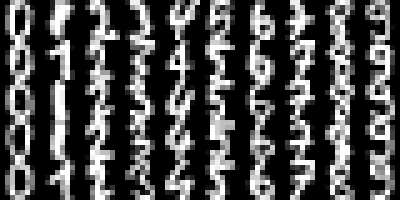
\includegraphics[width=0.9\linewidth]{../assets/digit_samples.png}
      \end{center}
    \end{column}
    \begin{column}{0.5\textwidth}
      \begin{itemize}
        \item Each sample is a tiny $8\times8$ grayscale digit.
        \item DocScan must turn the water-meter crop into the number it shows.
        \item Same task all week: input $8\times8$ image $\rightarrow$ one of 10 classes.
      \end{itemize}
      \keyidea{Keep this concrete task in mind --- every abstract idea today plugs straight into it.}
    \end{column}
  \end{columns}
\end{frame}

\begin{frame}{Convolution: you already know it}
  \begin{itemize}
    \item Week 3: slide a small kernel over the image, multiply-and-sum $\rightarrow$ a filtered image.
    \item A Sobel kernel detects edges; a blur kernel smooths. \emph{We} chose the numbers.
    \item A \term{convolutional layer} is the same operation --- but the kernel numbers are \term{learned}.
  \end{itemize}
  \keyidea{A CNN is ``convolution with kernels chosen by training instead of by hand.''}
\end{frame}

\begin{frame}{A convolution, by hand}
  Slide a $3\times3$ kernel over the highlighted patch and multiply-and-sum.
  \begin{columns}[T]
    \begin{column}{0.42\textwidth}
      \centering \small Input patch\\[3pt]
      \pixelgrid{ {2,0,1}, {4,1,0}, {2,3,1} }
    \end{column}
    \begin{column}{0.18\textwidth}
      \centering \small Kernel (Sobel-$x$)\\[3pt]
      \pixelgrid{ {1,0,-1}, {2,0,-2}, {1,0,-1} }
    \end{column}
    \begin{column}{0.40\textwidth}
      \begin{mathbox}[Multiply--sum]
        $2(1)+0+1(-1)$\\
        $+\,4(2)+0+0(-2)$\\
        $+\,2(1)+0+1(-1)$\\
        $=2-1+8+2-1 = \mathbf{10}$
      \end{mathbox}
    \end{column}
  \end{columns}
  \vspace{2pt}
  One output pixel $=10$. Repeat over every position to get the whole feature map.
\end{frame}

\begin{frame}{Padding and stride}
  \begin{columns}[T]
    \begin{column}{0.55\textwidth}
      \begin{itemize}
        \item \term{Padding}: add a border of zeros so the kernel can sit on edge pixels --- output stays the same size.
        \item \term{Stride}: how far the kernel hops each step. Stride 2 halves the output.
      \end{itemize}
      \begin{mathbox}
        $\displaystyle H_{\text{out}}=\left\lfloor\frac{H+2P-K}{S}\right\rfloor+1$
      \end{mathbox}
    \end{column}
    \begin{column}{0.45\textwidth}
      \begin{infobox}[Our digit conv]
        $H=8,\ K=3,\ P=1,\ S=1$:
        \[ \tfrac{8+2-3}{1}+1 = 8 \]
        so an $8\times8$ input stays $8\times8$. That ``same'' padding is what we use.
      \end{infobox}
    \end{column}
  \end{columns}
\end{frame}

\begin{frame}{What the network learns}
  \begin{center}
  
\includegraphics[width=0.7\linewidth]{../assets/learned_filters.png}
  \end{center}
  \begin{itemize}
    \item These are the 8 first-layer $3\times3$ filters our CNN \emph{learned} for digits.
    \item Nobody designed them --- gradient descent found edge/stroke detectors that help read digits.
    \item Early layers learn edges; deeper layers combine them into parts, then whole shapes.
  \end{itemize}
\end{frame}

\begin{frame}{Feature maps}
  \begin{itemize}
    \item Applying one learned filter to the image gives a \term{feature map}: where that pattern appears.
    \item A layer has many filters $\rightarrow$ many feature maps (a ``stack'' of pattern detectors).
    \item The next layer convolves over that stack, combining simple patterns into complex ones.
  \end{itemize}
  \begin{mathbox}
    Conv layer: input stack $\rightarrow$ (learned filters) $\rightarrow$ output stack of feature maps.
  \end{mathbox}
\end{frame}

\begin{frame}{From one image to a stack of maps}
  \begin{center}
  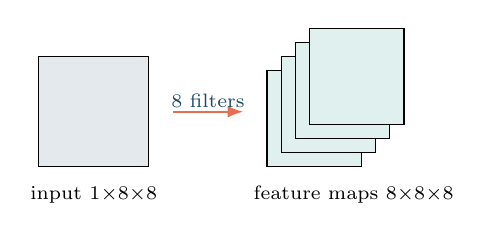
\begin{tikzpicture}[font=\scriptsize,every node/.style={inner sep=1pt}]
    % input
    \draw[fill=coursePrimary!12] (0,0) rectangle (1.4,1.4);
    \node at (0.7,-0.35) {input $1{\times}8{\times}8$};
    % arrow
    \draw[-{Latex[length=2mm]},thick,courseAccent] (1.7,0.7) -- (2.6,0.7)
      node[midway,above,coursePrimary]{8 filters};
    % output stack
    \foreach \i in {0,1,2,3} {
      \draw[fill=courseGood!15] (2.9+0.18*\i,0.18*\i) rectangle (4.1+0.18*\i,1.22+0.18*\i);
    }
    \node at (4.0,-0.35) {feature maps $8{\times}8{\times}8$};
  \end{tikzpicture}
  \end{center}
  \begin{itemize}
    \item Each of the 8 learned filters produces its own $8\times8$ map.
    \item Together they form a \term{tensor}: 8 channels of ``where this pattern is.''
    \item Depth = number of filters; height/width = spatial size after padding/stride.
  \end{itemize}
\end{frame}

% ==================================================================
\section{Anatomy of a CNN}
% ==================================================================

\begin{frame}{The building blocks}
  \begin{center}
  \begin{tabular}{@{}lll@{}}
    \toprule
    \textbf{Layer} & \textbf{Does} & \textbf{Why} \\
    \midrule
    Convolution & learned filters $\rightarrow$ feature maps & detect patterns \\
    ReLU & $\max(0,x)$, elementwise & add non-linearity \\
    Pooling & downsample (e.g. $2\times2$ max) & shrink, add invariance \\
    Fully-connected & flatten $\rightarrow$ class scores & make the decision \\
    Softmax & scores $\rightarrow$ probabilities & pick the class \\
    \bottomrule
  \end{tabular}
  \end{center}
  \keyidea{Conv+ReLU+Pool blocks stack up, ending in a classifier --- the standard CNN recipe.}
\end{frame}

\begin{frame}{The convolution layer, counted}
  A conv layer is defined by: \#input channels $C_{\text{in}}$, \#filters $C_{\text{out}}$, kernel $K\times K$.
  \begin{mathbox}[Weights in a conv layer]
    $\text{params} = C_{\text{out}}\big(C_{\text{in}}\cdot K\cdot K\big) + C_{\text{out}}$ \quad(the $+C_{\text{out}}$ is one bias per filter)
  \end{mathbox}
  \begin{itemize}
    \item Our first layer: $C_{\text{in}}{=}1,\ C_{\text{out}}{=}8,\ K{=}3 \Rightarrow 8(1\cdot9)+8 = \mathbf{80}$ weights.
    \item Crucial: the same 80 numbers are reused at \emph{every} pixel --- \term{weight sharing}.
  \end{itemize}
  \begin{goodbox}
    Weight sharing is why CNNs need far fewer parameters than a fully-connected net on pixels.
  \end{goodbox}
\end{frame}

\begin{frame}{Why ReLU (non-linearity)?}
  \begin{itemize}
    \item Stacking pure convolutions is still just one big linear filter --- no extra power.
    \item \term{ReLU} ($\max(0,x)$) inserts a non-linearity between layers.
    \item That lets deep stacks represent complex, curved decision boundaries.
  \end{itemize}
  \begin{mathbox}
    Without a non-linearity, ten conv layers collapse into one. ReLU is what makes ``deep'' meaningful.
  \end{mathbox}
\end{frame}

\begin{frame}{ReLU, by hand}
  ReLU clips every negative value to zero and leaves positives untouched.
  \begin{columns}[T]
    \begin{column}{0.44\textwidth}
      \centering \small Feature map (raw)\\[3pt]
      \pixelgrid{ {-3,5,-1}, {2,-4,0}, {7,-2,3} }
    \end{column}
    \begin{column}{0.12\textwidth}
      \centering\vspace{18pt}$\rightarrow$
    \end{column}
    \begin{column}{0.44\textwidth}
      \centering \small After ReLU\\[3pt]
      \pixelgrid{ {0,5,0}, {2,0,0}, {7,0,3} }
    \end{column}
  \end{columns}
  \vspace{4pt}
  \begin{itemize}
    \item Negatives $\rightarrow$ 0; positives pass through. Cheap and fast.
    \item Keeps only the ``this pattern is present'' evidence, discards the rest.
  \end{itemize}
\end{frame}

\begin{frame}{Why pooling?}
  \begin{itemize}
    \item \term{Max-pooling} keeps the strongest response in each small window, halving the size.
    \item Gives \term{translation tolerance}: a digit shifted a pixel still activates the same units.
    \item Shrinks computation and grows the \term{receptive field} of later layers.
  \end{itemize}
  \begin{goodbox}
    Pooling = ``I saw this pattern somewhere in this region,'' not ``exactly at this pixel.''
  \end{goodbox}
\end{frame}

\begin{frame}{Max-pooling, by hand}
  Split into $2\times2$ windows; keep the max of each.
  \begin{columns}[T]
    \begin{column}{0.5\textwidth}
      \centering \small $4\times4$ feature map\\[3pt]
      \pixelgrid{ {1,3,2,0}, {4,2,1,5}, {0,1,6,2}, {2,3,1,0} }
    \end{column}
    \begin{column}{0.1\textwidth}
      \centering\vspace{26pt}$\rightarrow$
    \end{column}
    \begin{column}{0.35\textwidth}
      \centering \small $2\times2$ pooled\\[3pt]
      \pixelgrid{ {4,5}, {3,6} }
      \vspace{4pt}\\
      \scriptsize top-left window $\max(1,3,4,2)=4$
    \end{column}
  \end{columns}
  \vspace{2pt}
  Four numbers become one; the map shrinks $4\times4\rightarrow2\times2$, keeping the strongest signals.
\end{frame}

\begin{frame}{Receptive field: seeing more with depth}
  \begin{center}
  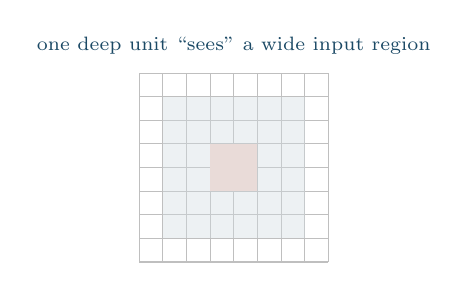
\begin{tikzpicture}[font=\scriptsize]
    \draw[step=0.3,gray!50] (0,0) grid (2.4,2.4);
    \fill[courseAccent!25] (0.9,0.9) rectangle (1.5,1.5); % after 1 conv
    \fill[coursePrimary!20,opacity=0.4] (0.3,0.3) rectangle (2.1,2.1); % after pool+conv
    \node[coursePrimary] at (1.2,2.75) {one deep unit ``sees'' a wide input region};
  \end{tikzpicture}
  \end{center}
  \begin{itemize}
    \item A unit after one $3\times3$ conv sees a $3\times3$ patch (coral).
    \item After a pool + another conv it sees a much larger region (blue).
    \item Deep units integrate whole-digit context, even though every kernel is tiny.
  \end{itemize}
\end{frame}

\begin{frame}{Fully-connected + softmax: the decision}
  \begin{itemize}
    \item \term{Flatten}: unroll the final map stack into one long vector.
    \item \term{Fully-connected} layer: every input times a weight $\rightarrow$ 10 raw scores (\term{logits}).
    \item \term{Softmax}: turn the 10 logits into probabilities that sum to 1.
  \end{itemize}
  \begin{mathbox}
    $\displaystyle p_i = \frac{e^{z_i}}{\sum_j e^{z_j}}$ \quad --- biggest logit becomes the most probable class.
  \end{mathbox}
\end{frame}

\begin{frame}{Our digit CNN, end to end}
  \begin{itemize}
    \item Input $8\times8$ digit $\rightarrow$ Conv(8 filters)+ReLU+Pool $\rightarrow$ $4\times4$.
    \item $\rightarrow$ Conv(16 filters)+ReLU+Pool $\rightarrow$ $2\times2$ $\rightarrow$ flatten (64) $\rightarrow$ FC $\rightarrow$ 10 scores.
    \item Softmax turns the 10 scores into probabilities; the largest is the predicted digit.
  \end{itemize}
  \keyidea{Two conv blocks and one linear layer --- tiny by modern standards, yet it reads digits at 97\%.}
\end{frame}

\begin{frame}{Shape bookkeeping (track the tensor)}
  \begin{center}
  \begin{tabular}{@{}lll@{}}
    \toprule
    \textbf{Stage} & \textbf{Output shape} $(C\times H\times W)$ & \textbf{Size change} \\
    \midrule
    Input            & $1\times8\times8$   & --- \\
    Conv1 (8, pad 1) & $8\times8\times8$   & depth $1\to8$ \\
    Pool ($2\times2$)& $8\times4\times4$   & spatial halved \\
    Conv2 (16, pad 1)& $16\times4\times4$  & depth $8\to16$ \\
    Pool ($2\times2$)& $16\times2\times2$  & spatial halved \\
    Flatten          & $64$ vector         & $16\cdot2\cdot2$ \\
    FC               & $10$ scores         & one per digit \\
    \bottomrule
  \end{tabular}
  \end{center}
  \keyidea{Spatial size shrinks, depth grows: the net trades ``where'' for ``what.''}
\end{frame}

\begin{frame}{Parameter budget of the digit CNN}
  \begin{center}
  \begin{tabular}{@{}lcc@{}}
    \toprule
    \textbf{Layer} & \textbf{Formula} & \textbf{Params} \\
    \midrule
    Conv1 $(1{\to}8,\ 3{\times}3)$  & $8(1\cdot9)+8$   & 80 \\
    Conv2 $(8{\to}16,\ 3{\times}3)$ & $16(8\cdot9)+16$ & 1{,}168 \\
    FC $(64{\to}10)$                & $64\cdot10+10$   & 650 \\
    \midrule
    \textbf{Total} & & \textbf{1{,}898} \\
    \bottomrule
  \end{tabular}
  \end{center}
  \begin{itemize}
    \item Under 2{,}000 numbers --- a fully-connected net on $8\times8$ pixels to 10 classes would already have 650.
    \item Weight sharing keeps the conv layers astonishingly cheap.
  \end{itemize}
\end{frame}

% ==================================================================
\section{In-class exercise}
% ==================================================================

\begin{frame}{\faPen~In-class exercise (10 min)}
  \begin{infobox}[Reason about the machine you just built]
  \end{infobox}
  \begin{enumerate}
    \item How is a convolutional layer related to the Sobel kernel from Week 3?
    \item Convolve the kernel $\left(\begin{smallmatrix}0&1\\1&0\end{smallmatrix}\right)$ over the patch $\left(\begin{smallmatrix}3&5\\2&4\end{smallmatrix}\right)$ at one position --- what is the output?
    \item A $16\times16$ input goes through Conv($K{=}3, P{=}1, S{=}1$) then $2\times2$ pool. What spatial size comes out?
    \item Why won't stacking convolutions \emph{without} ReLU give a more powerful model?
  \end{enumerate}
\end{frame}

\begin{frame}{\faPen~Debrief}
  \begin{itemize}
    \item (1) Both convolve a small kernel over the image; Sobel's numbers are fixed, the CNN's are \term{learned}.
    \item (2) $0\cdot3+1\cdot5+1\cdot2+0\cdot4 = 7$.
    \item (3) Conv with same padding keeps $16\times16$; the $2\times2$ pool halves it to $8\times8$.
    \item (4) Composing linear operations is still linear --- \term{ReLU}'s non-linearity is what adds power.
  \end{itemize}
  \keyidea{You can now trace an image through every layer and predict its shape --- the core CNN skill.}
\end{frame}

% ==================================================================
\section{Wrap-up}
% ==================================================================

\begin{frame}{Common pitfalls when reasoning about CNNs}
  \begin{badbox}[Watch out]
    \begin{itemize}
      \item Forgetting the bias term when counting parameters (one per filter, one per output unit).
      \item Confusing \emph{depth} (number of filters) with \emph{spatial} size (height/width).
      \item Assuming pooling ``loses everything'' --- it keeps the strongest evidence per region.
      \item Expecting more layers to help \emph{without} a non-linearity between them.
    \end{itemize}
  \end{badbox}
\end{frame}

\begin{frame}{Good habits}
  \begin{goodbox}
    \begin{itemize}
      \item Sketch the tensor shape after \emph{every} layer before you write code.
      \item Prefer ``same'' padding ($P=\lfloor K/2\rfloor$) when you want to control size only via pooling.
      \item Think of a conv layer as a bank of tiny pattern detectors reused everywhere.
    \end{itemize}
  \end{goodbox}
\end{frame}

\begin{frame}{What you can already do}
  \begin{itemize}
    \item Explain a convolutional layer as convolution with \emph{learned} filters + weight sharing.
    \item Compute an output pixel, an output size, a ReLU, and a max-pool by hand.
    \item Trace a tensor's shape and count parameters through a whole small CNN.
    \item Name every building block --- conv, ReLU, pool, FC, softmax --- and say why it is there.
  \end{itemize}
\end{frame}

\begin{frame}{Next session}
  \begin{alertblock}{Session 2 --- making the filters good}
    \begin{itemize}
      \item How the net \emph{learns} those filters: forward pass, loss, backprop, gradient descent.
      \item Cross-entropy and softmax with real numbers; learning rate, batches, epochs.
      \item Reading training curves; regularization; when CNNs beat classical ML.
      \item We train the digit reader to 97\% and ship it as the week's deliverable.
    \end{itemize}
  \end{alertblock}
  \emph{Come with today's architecture firmly in your head --- next time we bring it to life.}
\end{frame}

\begin{frame}[standout]
  A CNN is convolution with filters chosen by training.\\[4pt]
  \normalsize Today we built the machine: conv, ReLU, pooling, and a classifier. Next: we teach it.
\end{frame}

\end{document}
